\documentclass[tikz,border=12pt]{standalone}
\usepackage{tikz}
\usetikzlibrary{arrows.meta}

\definecolor{fairblue}{RGB}{33, 102, 172}
\definecolor{fairmidblue}{RGB}{103, 169, 207}
\definecolor{fairlight}{RGB}{247, 247, 247}
\definecolor{fairmidred}{RGB}{239, 138, 98}
\definecolor{fairred}{RGB}{178, 24, 43}
\definecolor{darkgray}{RGB}{60, 60, 60}
\definecolor{lightgrid}{RGB}{230, 230, 230}

\begin{document}
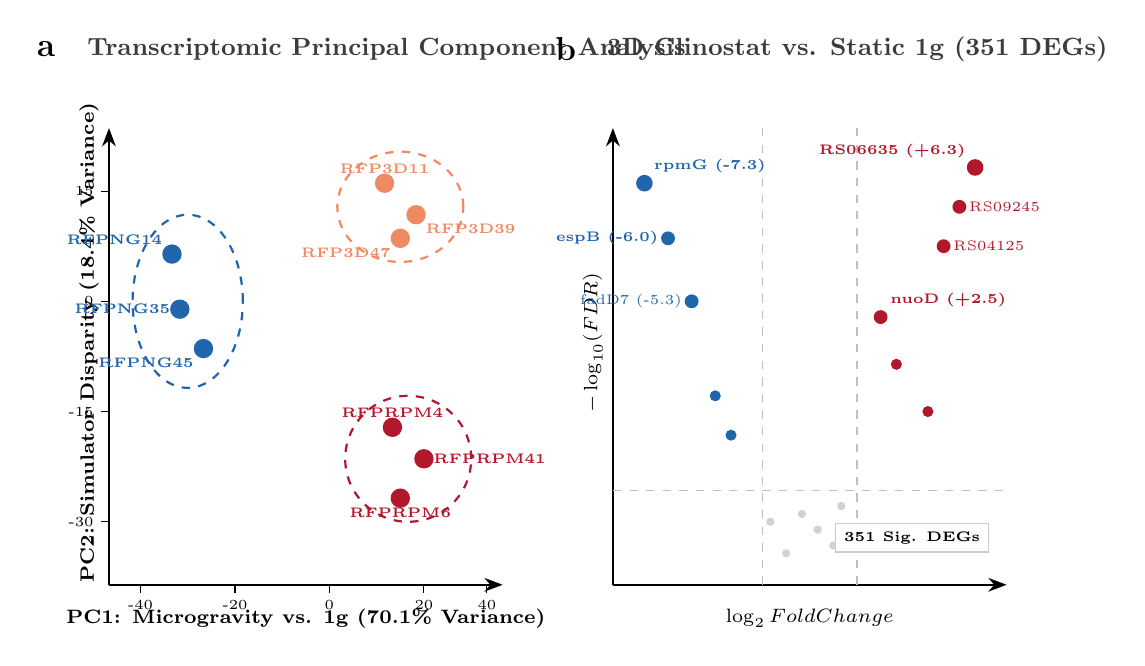
\begin{tikzpicture}[font=\sffamily, >=Stealth]
  % Panel a: PCA Biplot
  \node[font=\large\bfseries] at (0, 7.8) {a};
  \node[anchor=west, font=\small\bfseries, text=darkgray] at (0.4, 7.8) {Transcriptomic Principal Component Analysis};
  
  % Axes
  \draw[->, thick] (0.8, 1.0) -- (5.8, 1.0) node[midway, below=5pt, font=\scriptsize\bfseries] {PC1: Microgravity vs. 1g (70.1\% Variance)};
  \draw[->, thick] (0.8, 1.0) -- (0.8, 6.8) node[midway, above=5pt, rotate=90, font=\scriptsize\bfseries] {PC2: Simulator Disparity (18.4\% Variance)};

  % Axis Ticks
  \foreach \x/\lbl in {1.2/-40, 2.4/-20, 3.6/0, 4.8/20, 5.6/40} {
    \draw (\x, 0.9) -- (\x, 1.0) node[below=2pt, font=\tiny] {\lbl};
  }
  \foreach \y/\lbl in {1.8/-30, 3.2/-15, 4.6/0, 6.0/15} {
    \draw (0.7, \y) -- (0.8, \y) node[left=2pt, font=\tiny] {\lbl};
  }

  % Static 1g Points (Blue)
  \draw[thick, dashed, draw=fairblue] (1.8, 4.6) ellipse (0.7cm and 1.1cm);
  \fill[fairblue] (1.6, 5.2) circle (3.5pt) node[anchor=south east, font=\tiny\bfseries] {RFPNG14};
  \fill[fairblue] (1.7, 4.5) circle (3.5pt) node[anchor=east, font=\tiny\bfseries] {RFPNG35};
  \fill[fairblue] (2.0, 4.0) circle (3.5pt) node[anchor=north east, font=\tiny\bfseries] {RFPNG45};

  % 3D Clinostat Points (Mid-Red/Slate)
  \draw[thick, dashed, draw=fairmidred] (4.5, 5.8) ellipse (0.8cm and 0.7cm);
  \fill[fairmidred] (4.3, 6.1) circle (3.5pt) node[anchor=south, font=\tiny\bfseries] {RFP3D11};
  \fill[fairmidred] (4.7, 5.7) circle (3.5pt) node[anchor=north west, font=\tiny\bfseries] {RFP3D39};
  \fill[fairmidred] (4.5, 5.4) circle (3.5pt) node[anchor=north east, font=\tiny\bfseries] {RFP3D47};

  % RPM 2.0 Points (Deep Red)
  \draw[thick, dashed, draw=fairred] (4.6, 2.6) ellipse (0.8cm and 0.8cm);
  \fill[fairred] (4.4, 3.0) circle (3.5pt) node[anchor=south, font=\tiny\bfseries] {RFPRPM4};
  \fill[fairred] (4.8, 2.6) circle (3.5pt) node[anchor=west, font=\tiny\bfseries] {RFPRPM41};
  \fill[fairred] (4.5, 2.1) circle (3.5pt) node[anchor=north, font=\tiny\bfseries] {RFPRPM6};

  % Panel b: Volcano Plot 3D Clinostat vs 1g
  \node[font=\large\bfseries] at (6.6, 7.8) {b};
  \node[anchor=west, font=\small\bfseries, text=darkgray] at (7.0, 7.8) {3D Clinostat vs. Static 1g (351 DEGs)};
  
  \draw[->, thick] (7.2, 1.0) -- (12.2, 1.0) node[midway, below=5pt, font=\scriptsize\bfseries] {$\log_2\text{Fold Change}$};
  \draw[->, thick] (7.2, 1.0) -- (7.2, 6.8) node[midway, above=5pt, rotate=90, font=\scriptsize\bfseries] {$-\log_{10}(\text{FDR})$};

  % Threshold lines
  \draw[dashed, gray!50] (7.2, 2.2) -- (12.2, 2.2);
  \draw[dashed, gray!50] (9.1, 1.0) -- (9.1, 6.8);
  \draw[dashed, gray!50] (10.3, 1.0) -- (10.3, 6.8);

  % Non-sig scatter
  \foreach \x/\y in {9.4/1.4, 9.8/1.7, 9.6/1.9, 10.0/1.5, 9.2/1.8, 10.1/2.0} {
    \fill[gray!35] (\x, \y) circle (1.5pt);
  }
  % Upregulated (Deep Red)
  \fill[fairred] (11.8, 6.3) circle (3pt) node[anchor=south east, font=\tiny\bfseries] {RS06635 (+6.3)};
  \fill[fairred] (11.6, 5.8) circle (2.5pt) node[anchor=west, font=\tiny] {RS09245};
  \fill[fairred] (11.4, 5.3) circle (2.5pt) node[anchor=west, font=\tiny] {RS04125};
  \fill[fairred] (10.6, 4.4) circle (2.5pt) node[anchor=south west, font=\tiny\bfseries] {nuoD (+2.5)};
  \fill[fairred] (10.8, 3.8) circle (2pt);
  \fill[fairred] (11.2, 3.2) circle (2pt);

  % Downregulated (Deep Blue)
  \fill[fairblue] (7.6, 6.1) circle (3pt) node[anchor=south west, font=\tiny\bfseries] {rpmG (-7.3)};
  \fill[fairblue] (7.9, 5.4) circle (2.5pt) node[anchor=east, font=\tiny\bfseries] {espB (-6.0)};
  \fill[fairblue] (8.2, 4.6) circle (2.5pt) node[anchor=east, font=\tiny] {fadD7 (-5.3)};
  \fill[fairblue] (8.5, 3.4) circle (2pt);
  \fill[fairblue] (8.7, 2.9) circle (2pt);

  % Summary Badge
  \node[fill=white, draw=gray!40, font=\tiny\bfseries, inner sep=3pt] at (11.0, 1.6) {351 Sig. DEGs};
\end{tikzpicture}
\end{document}
